\chapter{Results}
In this chapter the results produced by the application of the different trading strategies are discussed, but first of all final instructions on the setup of the system are given. 
\section{Final Setup}
After the previously performed trading analysis in chapter \ref{chap:tradingDynamics} the configuration from scenario has been used in all further studies. The corresponding ini files can be found in the appendix in \ref{chap:iniContainment}. They resemble the description given in chapter \ref{chap:testedStrategiesDesc}.  
In order to keep the runtime reasonable for this thesis and testing, farms with a smaller size than 20 cows have been excluded from the simulation. The argument for this is that small farms can not build a sustainable business and are rather run by families, which want to make some money besides their daytime jobs. They will most likely not buy and sell cows all the time and therefore not play a big role in the spreading of BVD on the network. This assumption has not been proven by now. \citep{steinbach16} provided a categorisation of nodes based on their trading behavior as markets, traders, self-sustaining premises, fattening and breeding farms. This method could be refined to build a more realistic model of the market in the future. 
Applying this idea removes $15272\cows$ ($4.46\,\%$) in $5544\,\text{farms}$ ($82.16\,\%$).
Since the behavior of the different farms has not been studied and implemented in this simulation fully and because the system size in terms of farms is much smaller than the actual network size of all of Thuringia, the implementation of a more refined and realistic market behavior has been postponed. 
The data given in chapter \ref {chap:rlDataRegulationGermany} has been used to set up the system. This was done by randomly choosing $2\,\%$ of the farms to be set up with the shares of the different compartments of previously with PIs contaminated farms. The other $98\,\%$ of the farms were set up with the shares of all compartments corresponding to now previous contamination by PIs. With all these measures taken multiple simulations where run. The global prevalence strongly depends on the farms chosen to be infected in the beginning. If smaller farms are contaminated in the beginning, the disease will need much longer to spread or even die out, since far less animals are infected and the in- and out-degree of these small farms are relatively small, which leads to a smaller infection rate for all other nodes. With the aim of limiting the amount of scenarios to be discussed, one scenario which exposed a prevalence close to the big single farm with approximately $40000\cows$ from section \ref{chap:diseaseDynamicsDesc} has been chosen. It exhibited the highest global prevalence after $20\days$. The seed from this run is used in all runs for the different strategies, to make sure that the transients for the system for all strategies look exactly the same. By setting the seed of the random number generator, two streams of random numbers produced by this random number generator will be exactly the same. This is used to have the same events happen during the transient phase for all strategies, leading to results, which can be compared. The containment strategies in each scenario are turned on on a global scale after $10000\days$. The cows from the cow well farm still 
\section{Strategy I - No Strategy}
This first run corresponds to the control group in clinical tests of medication. As can be seen in figure \ref{fig:cont1Behav}, for some not entirely clear reason the number of recovered animals and therefore their share on the total population drops, giving rise to the number of susceptibles. 
\begin{figure}[htbp]
\begin{minipage}{0.5\textwidth}
\centering
\noindent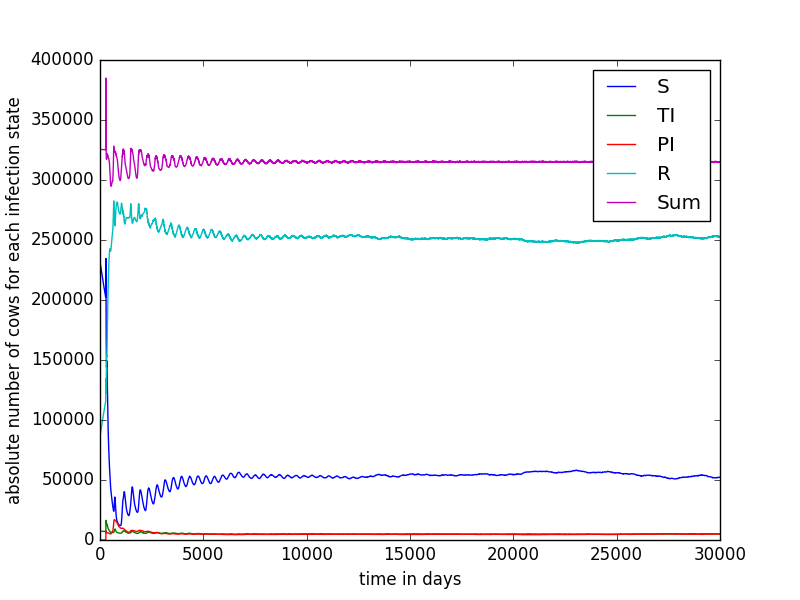
\includegraphics[width=0.95\linewidth,height=\textheight,
keepaspectratio]{cont1totalEndemicNumbers.png} 
\end{minipage}
\begin{minipage}{0.5\textwidth}
\centering
\noindent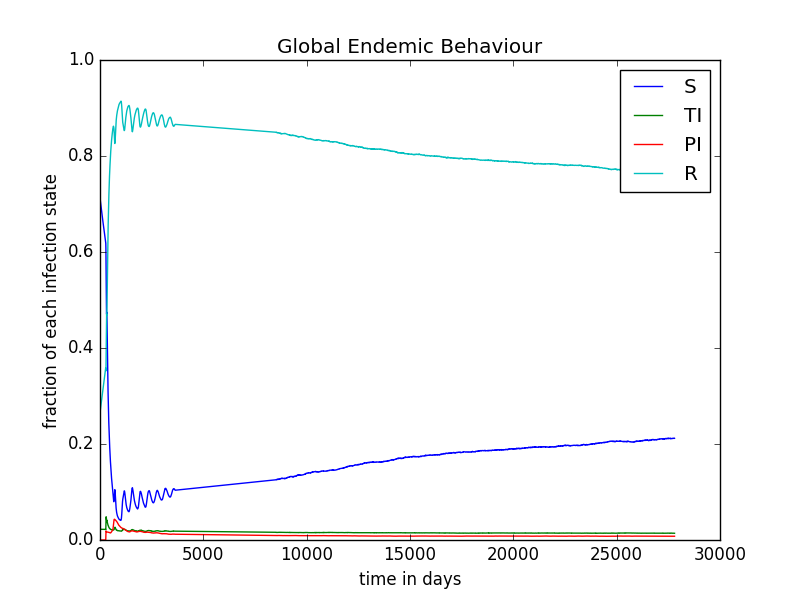
\includegraphics[width=0.95\linewidth,height=\textheight,
keepaspectratio]{cont1endemicFractions.png} 
\end{minipage}
\caption[Endemic Behavior in Containment Strategy One]{}
\label{fig:cont1Behav}
\end{figure} 
This all happens while the numbers of TIs and PIs stay stable. The sum stays stable, but starts to oscillate a little bit as the number of recovered starts to oscillate around $8000\days$. These oscillations express themselves in a slightly thicker line for both, the number of recovered animals and the sum of all compartments. The stable 

\section{Strategy II - Old BVD regulation}

\begin{figure}[htbp]
\begin{minipage}{0.5\textwidth}
\centering
\noindent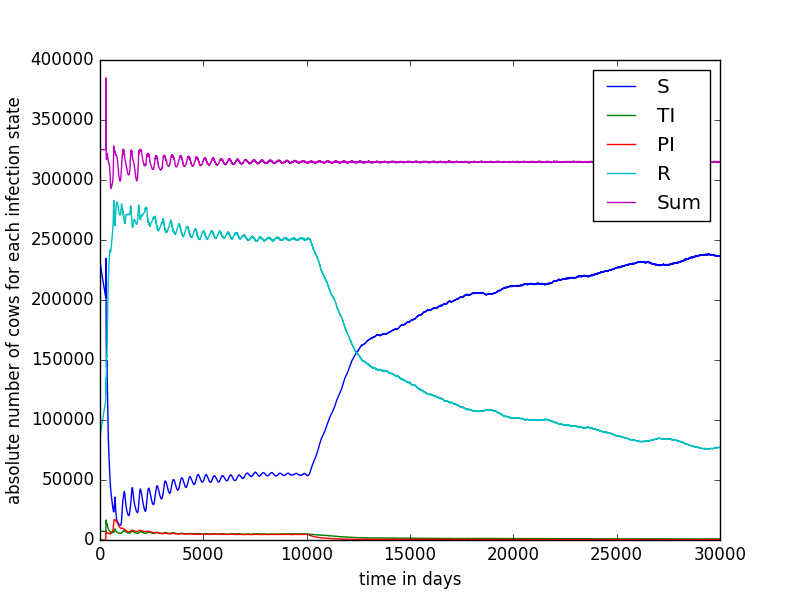
\includegraphics[width=0.95\linewidth,height=\textheight,
keepaspectratio]{cont2totalEndemicNumbers.png} 
\end{minipage}
\begin{minipage}{0.5\textwidth}
\centering
\noindent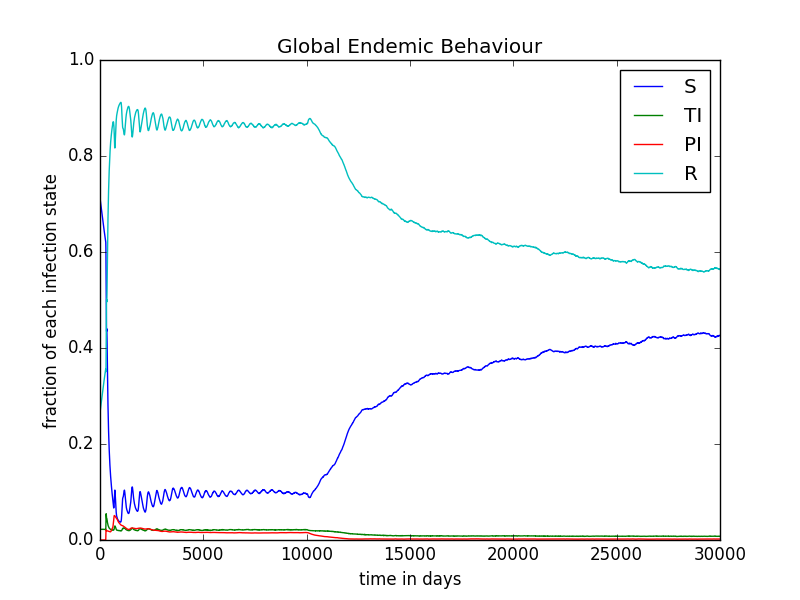
\includegraphics[width=0.95\linewidth,height=\textheight,
keepaspectratio]{cont2endemicFractions.png} 
\end{minipage}
\caption[Endemic Behavior in Containment Strategy One]{}
\label{fig:demographyScen8}
\end{figure}


\section{Strategy III - New BVD regulation}

\begin{figure}[htbp]
\begin{minipage}{0.5\textwidth}
\centering
\noindent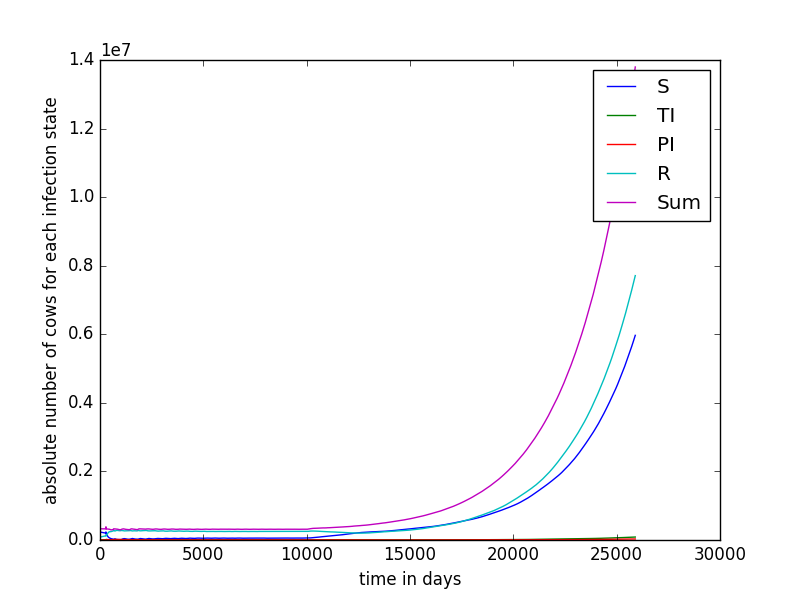
\includegraphics[width=0.95\linewidth,height=\textheight,
keepaspectratio]{cont3totalEndemicNumbers.png} 
\end{minipage}
\begin{minipage}{0.5\textwidth}
\centering
\noindent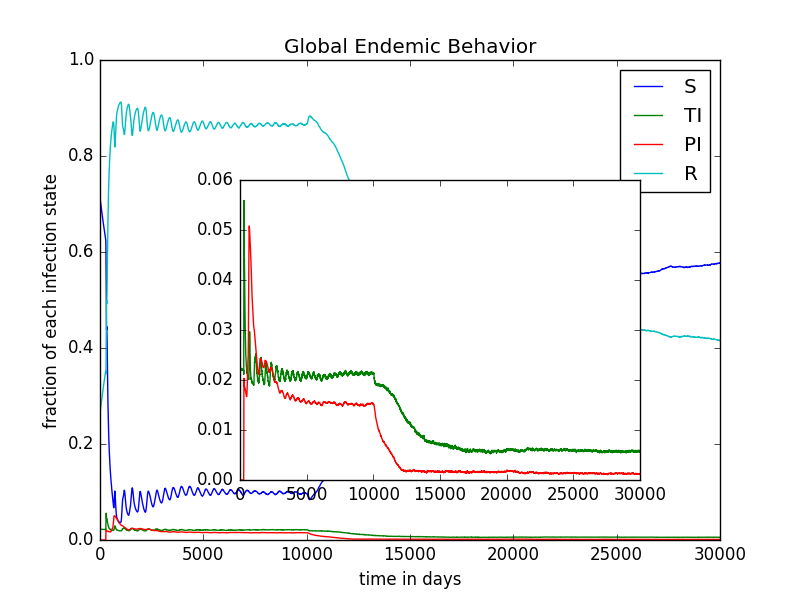
\includegraphics[width=0.95\linewidth,height=\textheight,
keepaspectratio]{cont3pendemicFractions.png} 
\end{minipage}
\caption[Endemic Behavior in Containment Strategy One]{}
\label{fig:demographyScen8}
\end{figure}


\section{Strategy IV - New BVD regulation + Vaccination}


\begin{figure}[htbp]
\begin{minipage}{0.5\textwidth}
\centering
\noindent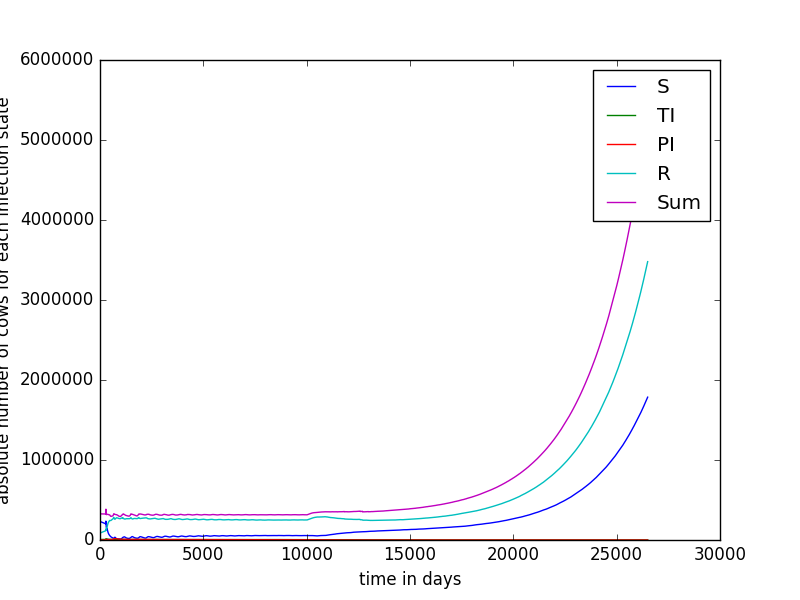
\includegraphics[width=0.95\linewidth,height=\textheight,
keepaspectratio]{cont4totalEndemicNumbers.png} 
\end{minipage}
\begin{minipage}{0.5\textwidth}
\centering
\noindent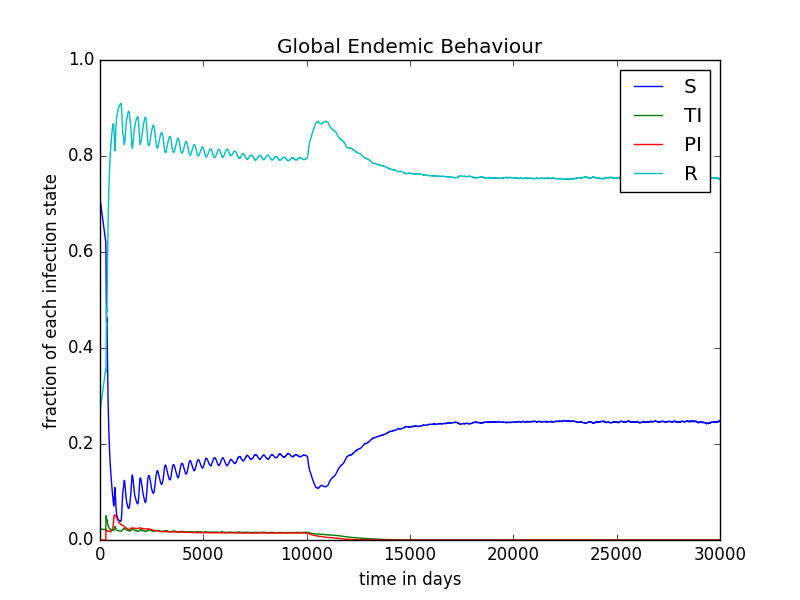
\includegraphics[width=0.95\linewidth,height=\textheight,
keepaspectratio]{cont4endemicFractions.png} 
\end{minipage}
\caption[Endemic Behavior in Containment Strategy One]{}
\label{fig:demographyScen8}
\end{figure}


\section{Strategy V - New BVD regulation + young calf window}
\subsection{Strategy Va}

\begin{figure}[htbp]
\begin{minipage}{0.5\textwidth}
\centering
\noindent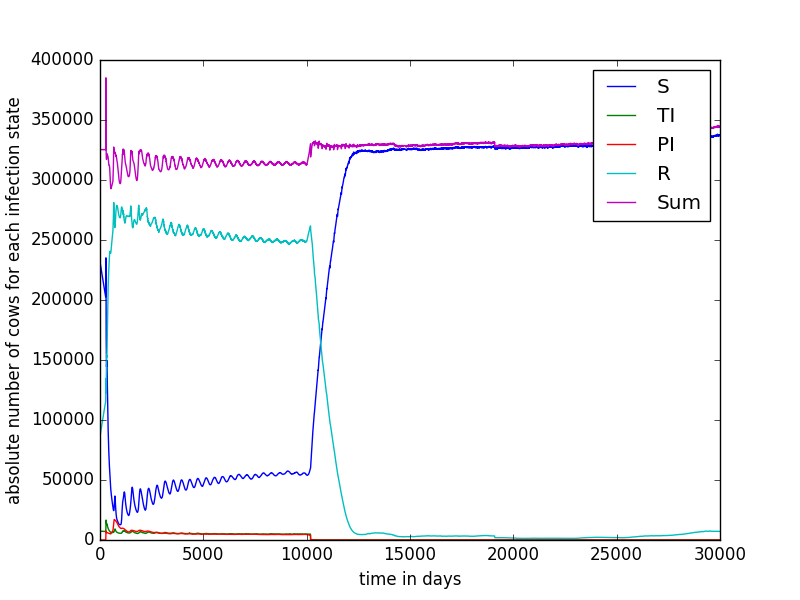
\includegraphics[width=0.95\linewidth,height=\textheight,
keepaspectratio]{cont5totalEndemicNumbers.png} 
\end{minipage}
\begin{minipage}{0.5\textwidth}
\centering
\noindent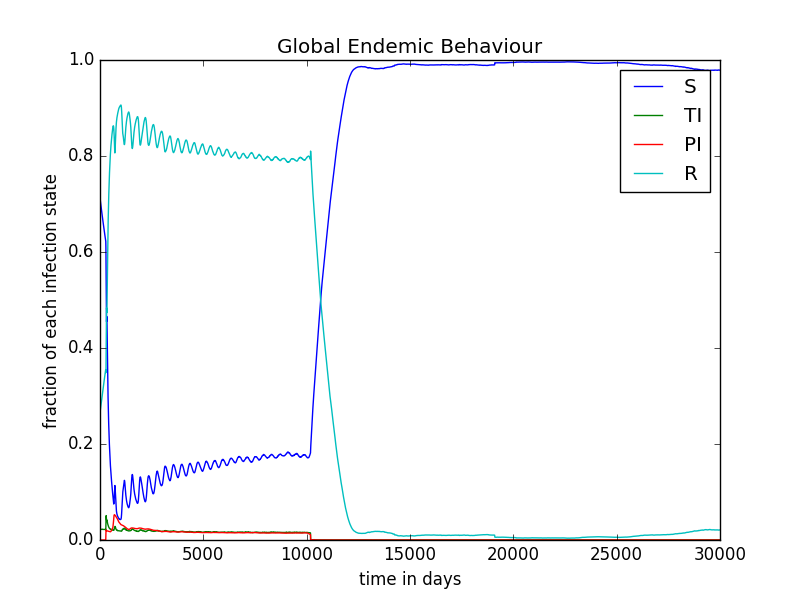
\includegraphics[width=0.95\linewidth,height=\textheight,
keepaspectratio]{cont5endemicFractions.png} 
\end{minipage}
\caption[Endemic Behavior in Containment Strategy One]{}
\label{fig:demographyScen8}
\end{figure}

\subsection{Strategy Vb}

\begin{figure}[htbp]
\begin{minipage}{0.5\textwidth}
\centering
\noindent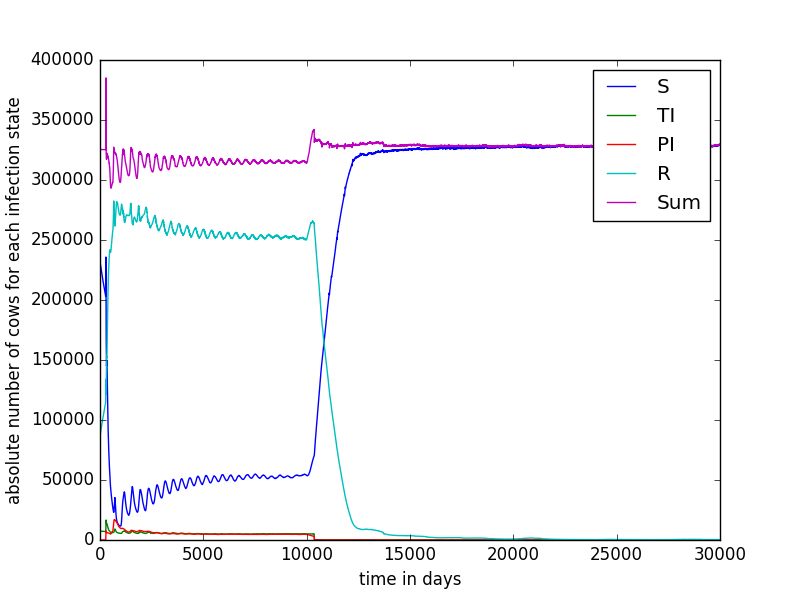
\includegraphics[width=0.95\linewidth,height=\textheight,
keepaspectratio]{cont5btotalEndemicNumbers.png} 
\end{minipage}
\begin{minipage}{0.5\textwidth}
\centering
\noindent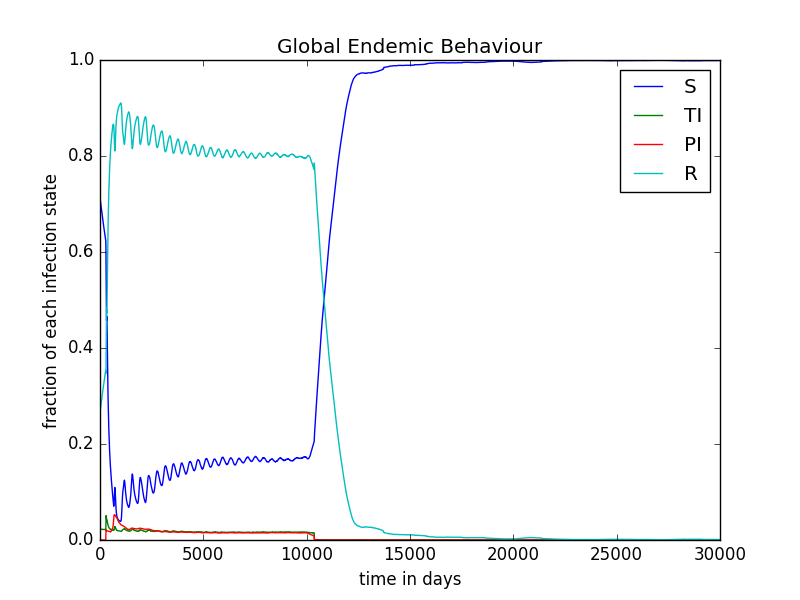
\includegraphics[width=0.95\linewidth,height=\textheight,
keepaspectratio]{cont5bendemicFractions.png} 
\end{minipage}
\caption[Endemic Behavior in Containment Strategy One]{}
\label{fig:demographyScen8}
\end{figure}

\section{Strategy VI - New BVD regulation + Vaccination + young calf window} 
\subsection{Strategy VIa}

\begin{figure}[htbp]
\begin{minipage}{0.5\textwidth}
\centering
\noindent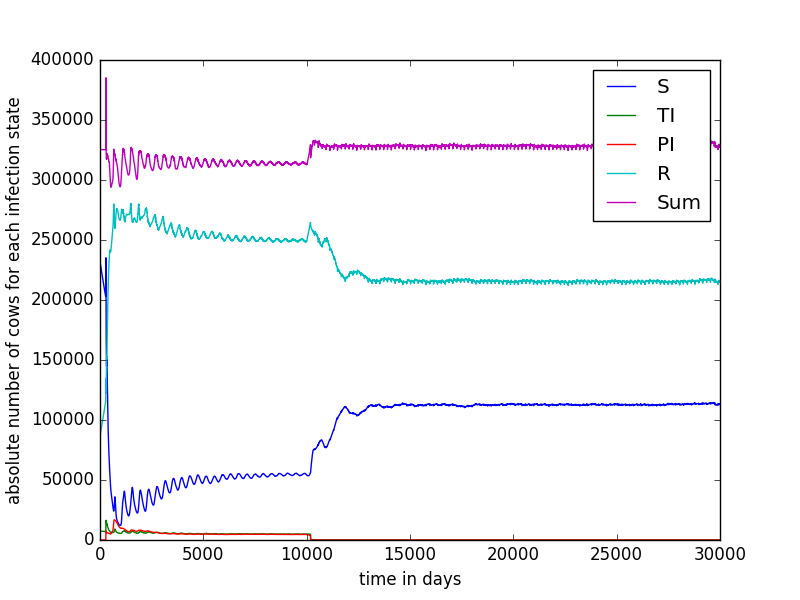
\includegraphics[width=0.95\linewidth,height=\textheight,
keepaspectratio]{cont6totalEndemicNumbers.png} 
\end{minipage}
\begin{minipage}{0.5\textwidth}
\centering
\noindent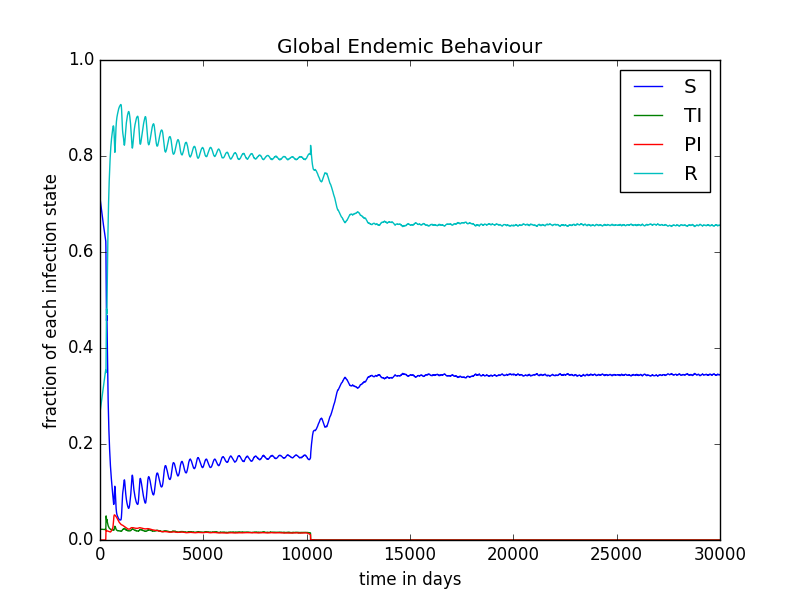
\includegraphics[width=0.95\linewidth,height=\textheight,
keepaspectratio]{cont6endemicFractions.png} 
\end{minipage}
\caption[Endemic Behavior in Containment Strategy One]{}
\label{fig:demographyScen8}
\end{figure}

\subsection{Strategy VIb}

\begin{figure}[htbp]
\begin{minipage}{0.5\textwidth}
\centering
\noindent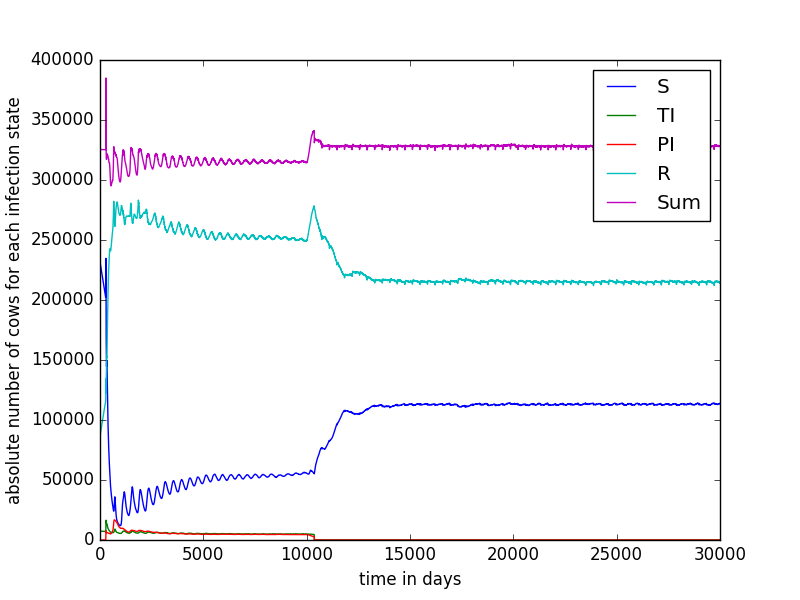
\includegraphics[width=0.95\linewidth,height=\textheight,
keepaspectratio]{cont6btotalEndemicNumbers.png} 
\end{minipage}
\begin{minipage}{0.5\textwidth}
\centering
\noindent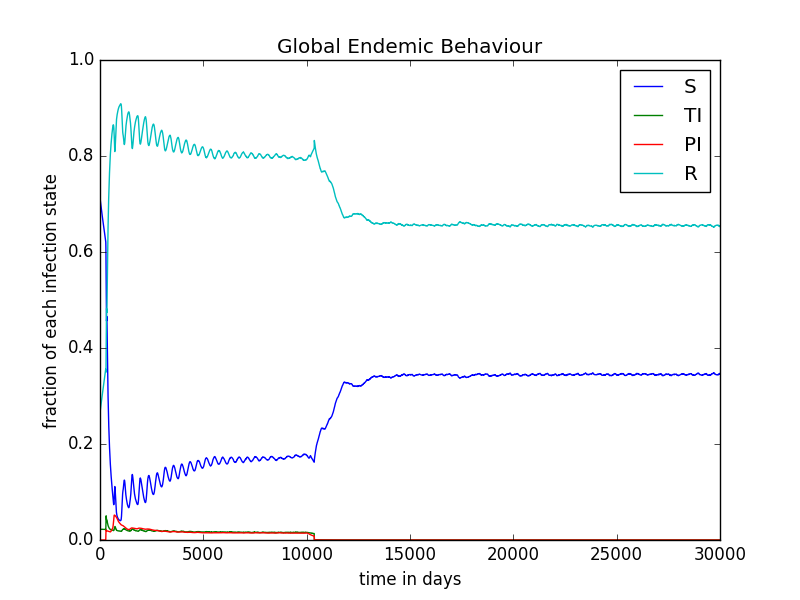
\includegraphics[width=0.95\linewidth,height=\textheight,
keepaspectratio]{cont6bendemicFractions.png} 
\end{minipage}
\caption[Endemic Behavior in Containment Strategy One]{}
\label{fig:demographyScen8}
\end{figure}

\section{Comparison of the different Strategies}